
\section{Datos: fuente y forma}
Los datos escogidos provienen del dataset \href{https://www.kaggle.com/chaitanyakck/medical-text}{Medical Text} publicado por Chaitanya Krishna Kasaraneni, y de \href{https://www.kaggle.com/tboyle10/medicaltranscriptions}{Medical Transcriptions}, publicado por Tara Boyle. La naturaleza de los mismos es ligeramente diferente así que explicaremos el proceso de preprocesamiento y unificación posteriormente.

En la Figura \ref{fig:preprocess-diagram} podemos ver un pequeño resumen del preprocesamiento que se acometerá a los datos. En la siguiente sección se detallan cada uno de estos pasos.

\subsection{Dataset: \textit{Medical Text}}
El dataset tiene formato \jesitt{.dat}, estructurado como un \jesitt{.tsv} (Tab Separated Values). La primera columna corresponde con una categoría determinada --ya que el dataset estaba diseñado para clasificación-- y la segunda columna contiene fragmentos de documentos médicos.

El dataset es en inglés, está anonimizado y los comentarios principalmente consisten en descripciones quirúrgicas o relacionadas con operaciones complejas. Podemos ver los dos primeros de nuestro conjunto de datos en los Comentarios \ref{com:com1} y \ref{com:com2}.

\begin{thm}
	\sffamily{
		Excision of limbal dermoids. We reviewed the clinical files of 10 patients who had undergone excision of unilateral epibulbar limbal dermoids. Preoperatively, all of the affected eyes had worse visual acuity (P less than .02) and more astigmatism (P less than .01) than the contralateral eyes. Postoperatively, every patient was cosmetically improved. Of the eight patients for whom both preoperative and postoperative visual acuity measurements had been obtained, in six it had changed minimally (less than or equal to 1 line), and in two it had improved (less than or equal to 2 lines). Surgical complications included persistent epithelial defects (40\%) and peripheral corneal vascularization and opacity (70\%). These complications do not outweigh the cosmetic and visual benefits of dermoid excision in selected patients. 
	}
	\label{com:com1}
\end{thm}
\begin{thm}
	\sffamily{
		Retained endobronchial foreign body removal facilitated by steroid therapy of an obstructing, inflammatory polyp. Oral and topical steroids were used to induce regression in an inflammatory, obstructing endobronchial polyp caused by a retained foreign body. The FB (a peanut half), which had been present for over six months, was then able to be easily and bloodlessly retrieved with fiberoptic bronchoscopy. 
	}
	\label{com:com2}
\end{thm}

El dataset está descompuesto en un archivo \jesitt{train.dat} y otro \jesitt{test.dat}. El archivo de entrenamiento contiene 14438 comentarios, y el de evaluación, 14442. En total, disponemos de 28880 comentarios.

Como podemos observar en las Figuras \ref{fig:avg_char_train} y \ref{fig:avg_tokens_train}, la distribución de los distintos elementos de nuestro dataset de entrenamiento está muy normalmente distribuída.

El número medio de caracteres por comentario es de 1230, y el número medio de tokens por comentario es de unos 180, correspondiéndose con las líneas amarillas en las figuras.

Se pueden apreciar, aún así, algunos valores atípicos de comentarios particularmente largos. Esto, sin embargo, no es necesariamente malo en nuestro caso. En definitiva, cuanto más texto tengamos a nuestra disposición, mejor para el modelo.

\begin{figure}[h!]
	\centering
	\begin{subfigure}[t]{0.95\textwidth}
		\centering
		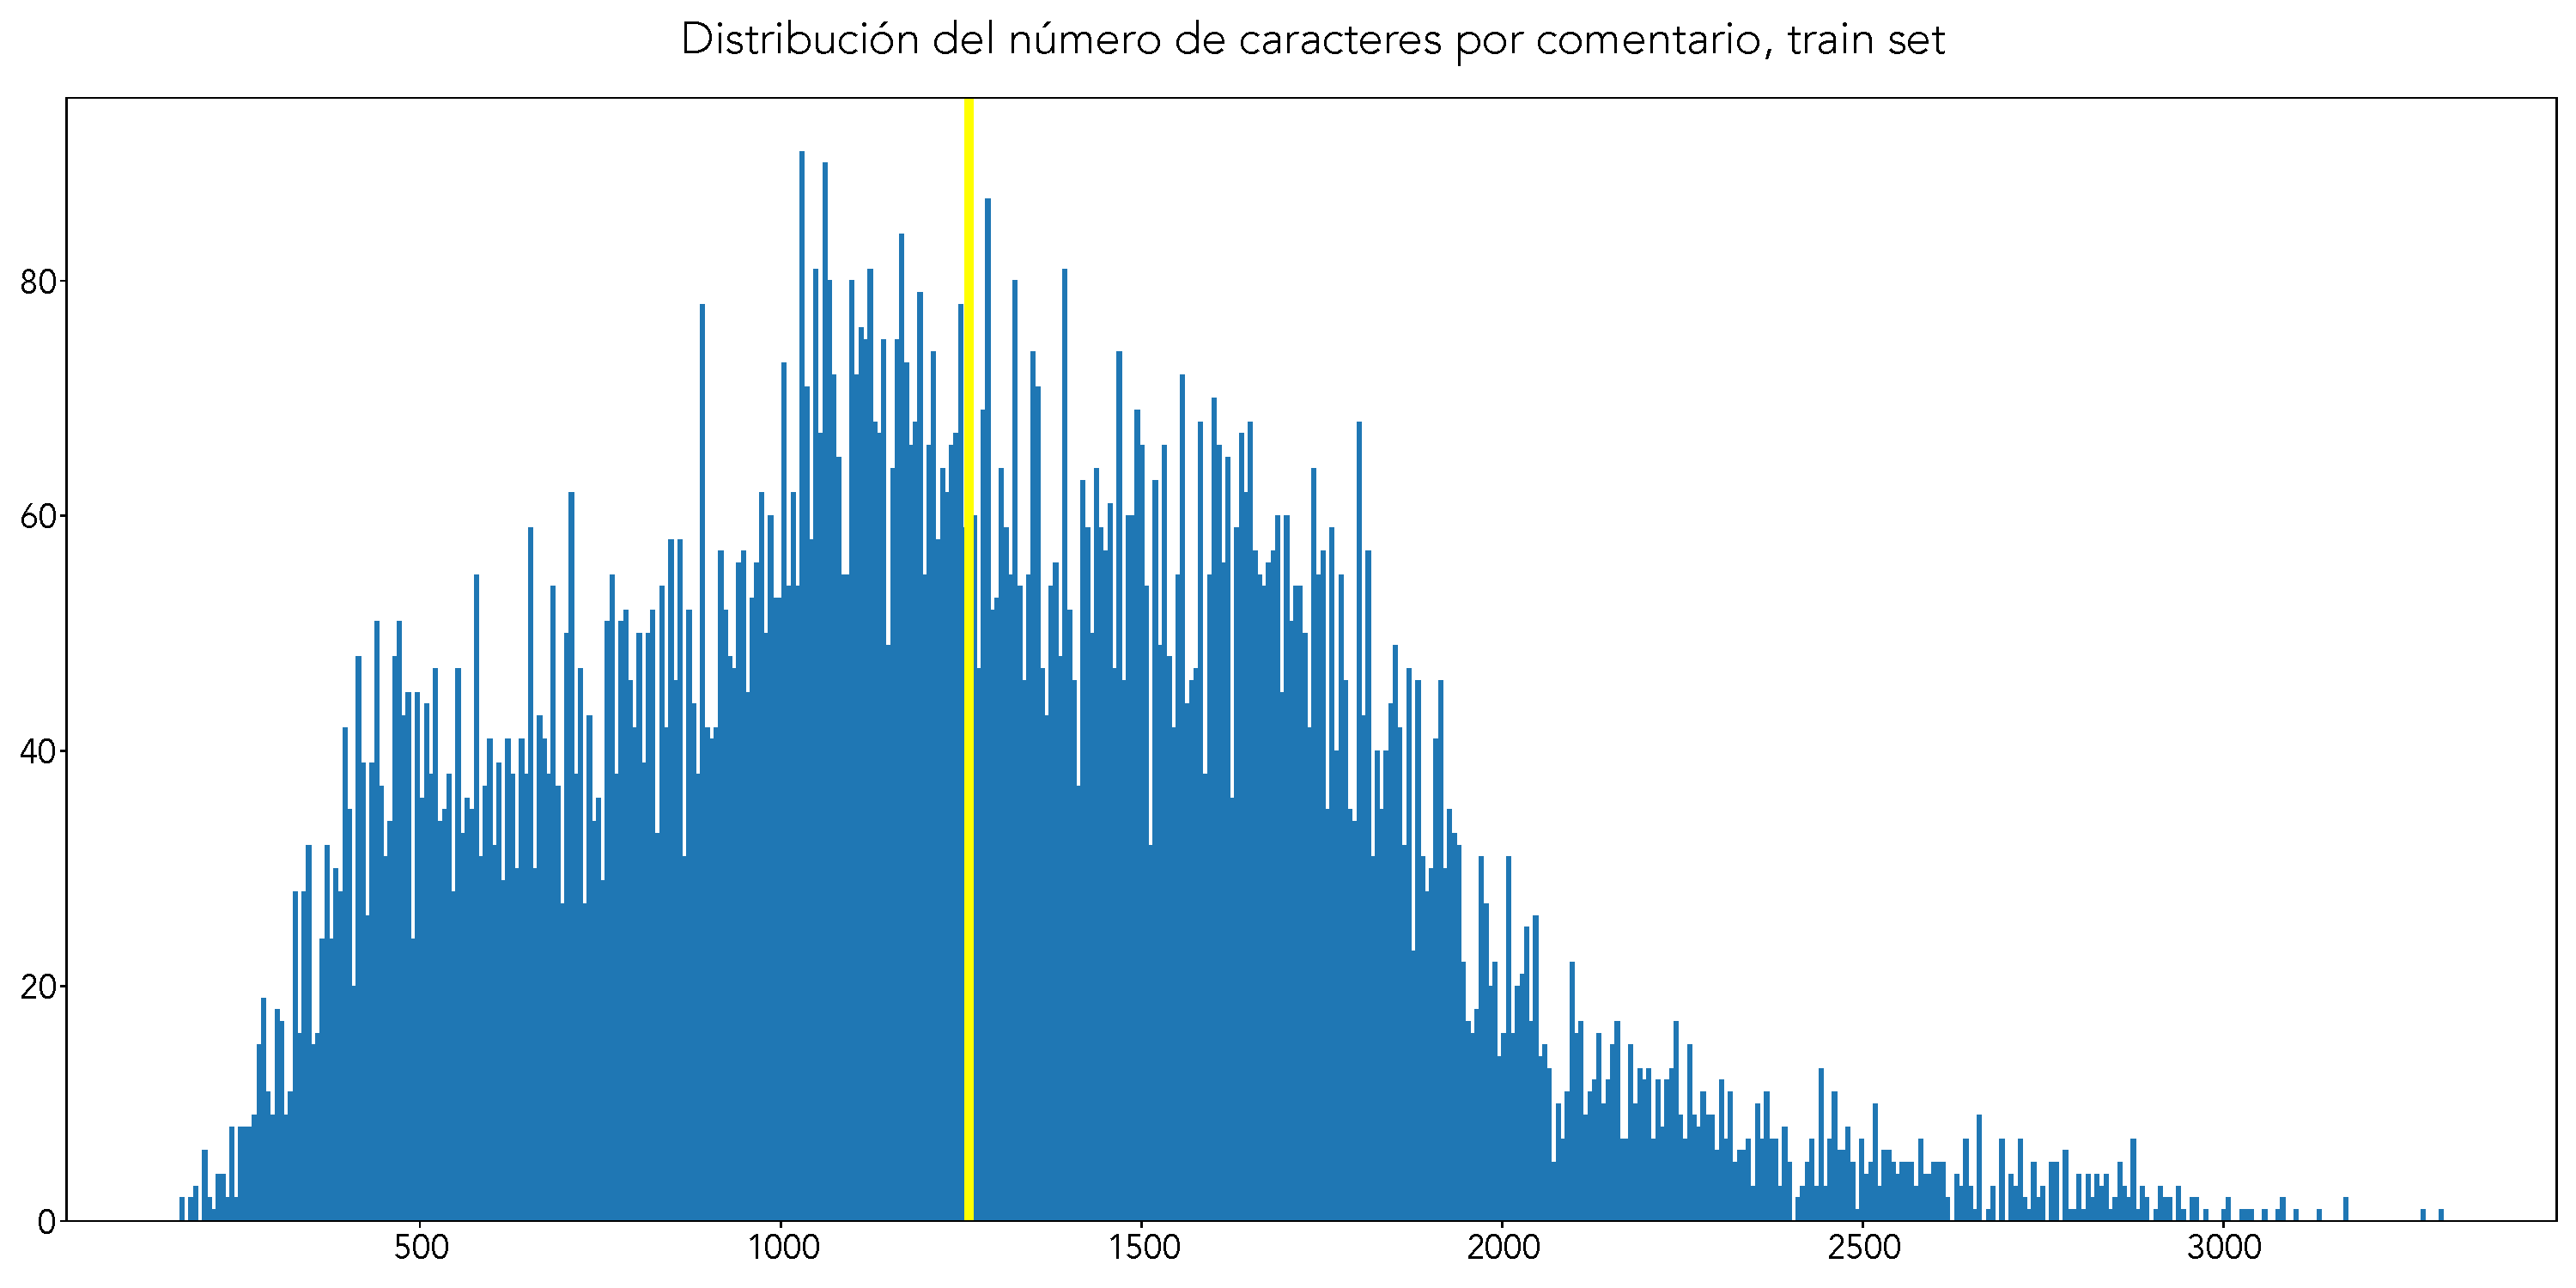
\includegraphics[width=.9\textwidth]{media/char_hist_train.pdf}
		\caption{Distribución del número de caracteres por comentario, en el conjunto de entrenamiento}
		\label{fig:avg_char_train}
	\end{subfigure}
	~

	\begin{subfigure}[t]{0.95\textwidth}
		\centering
		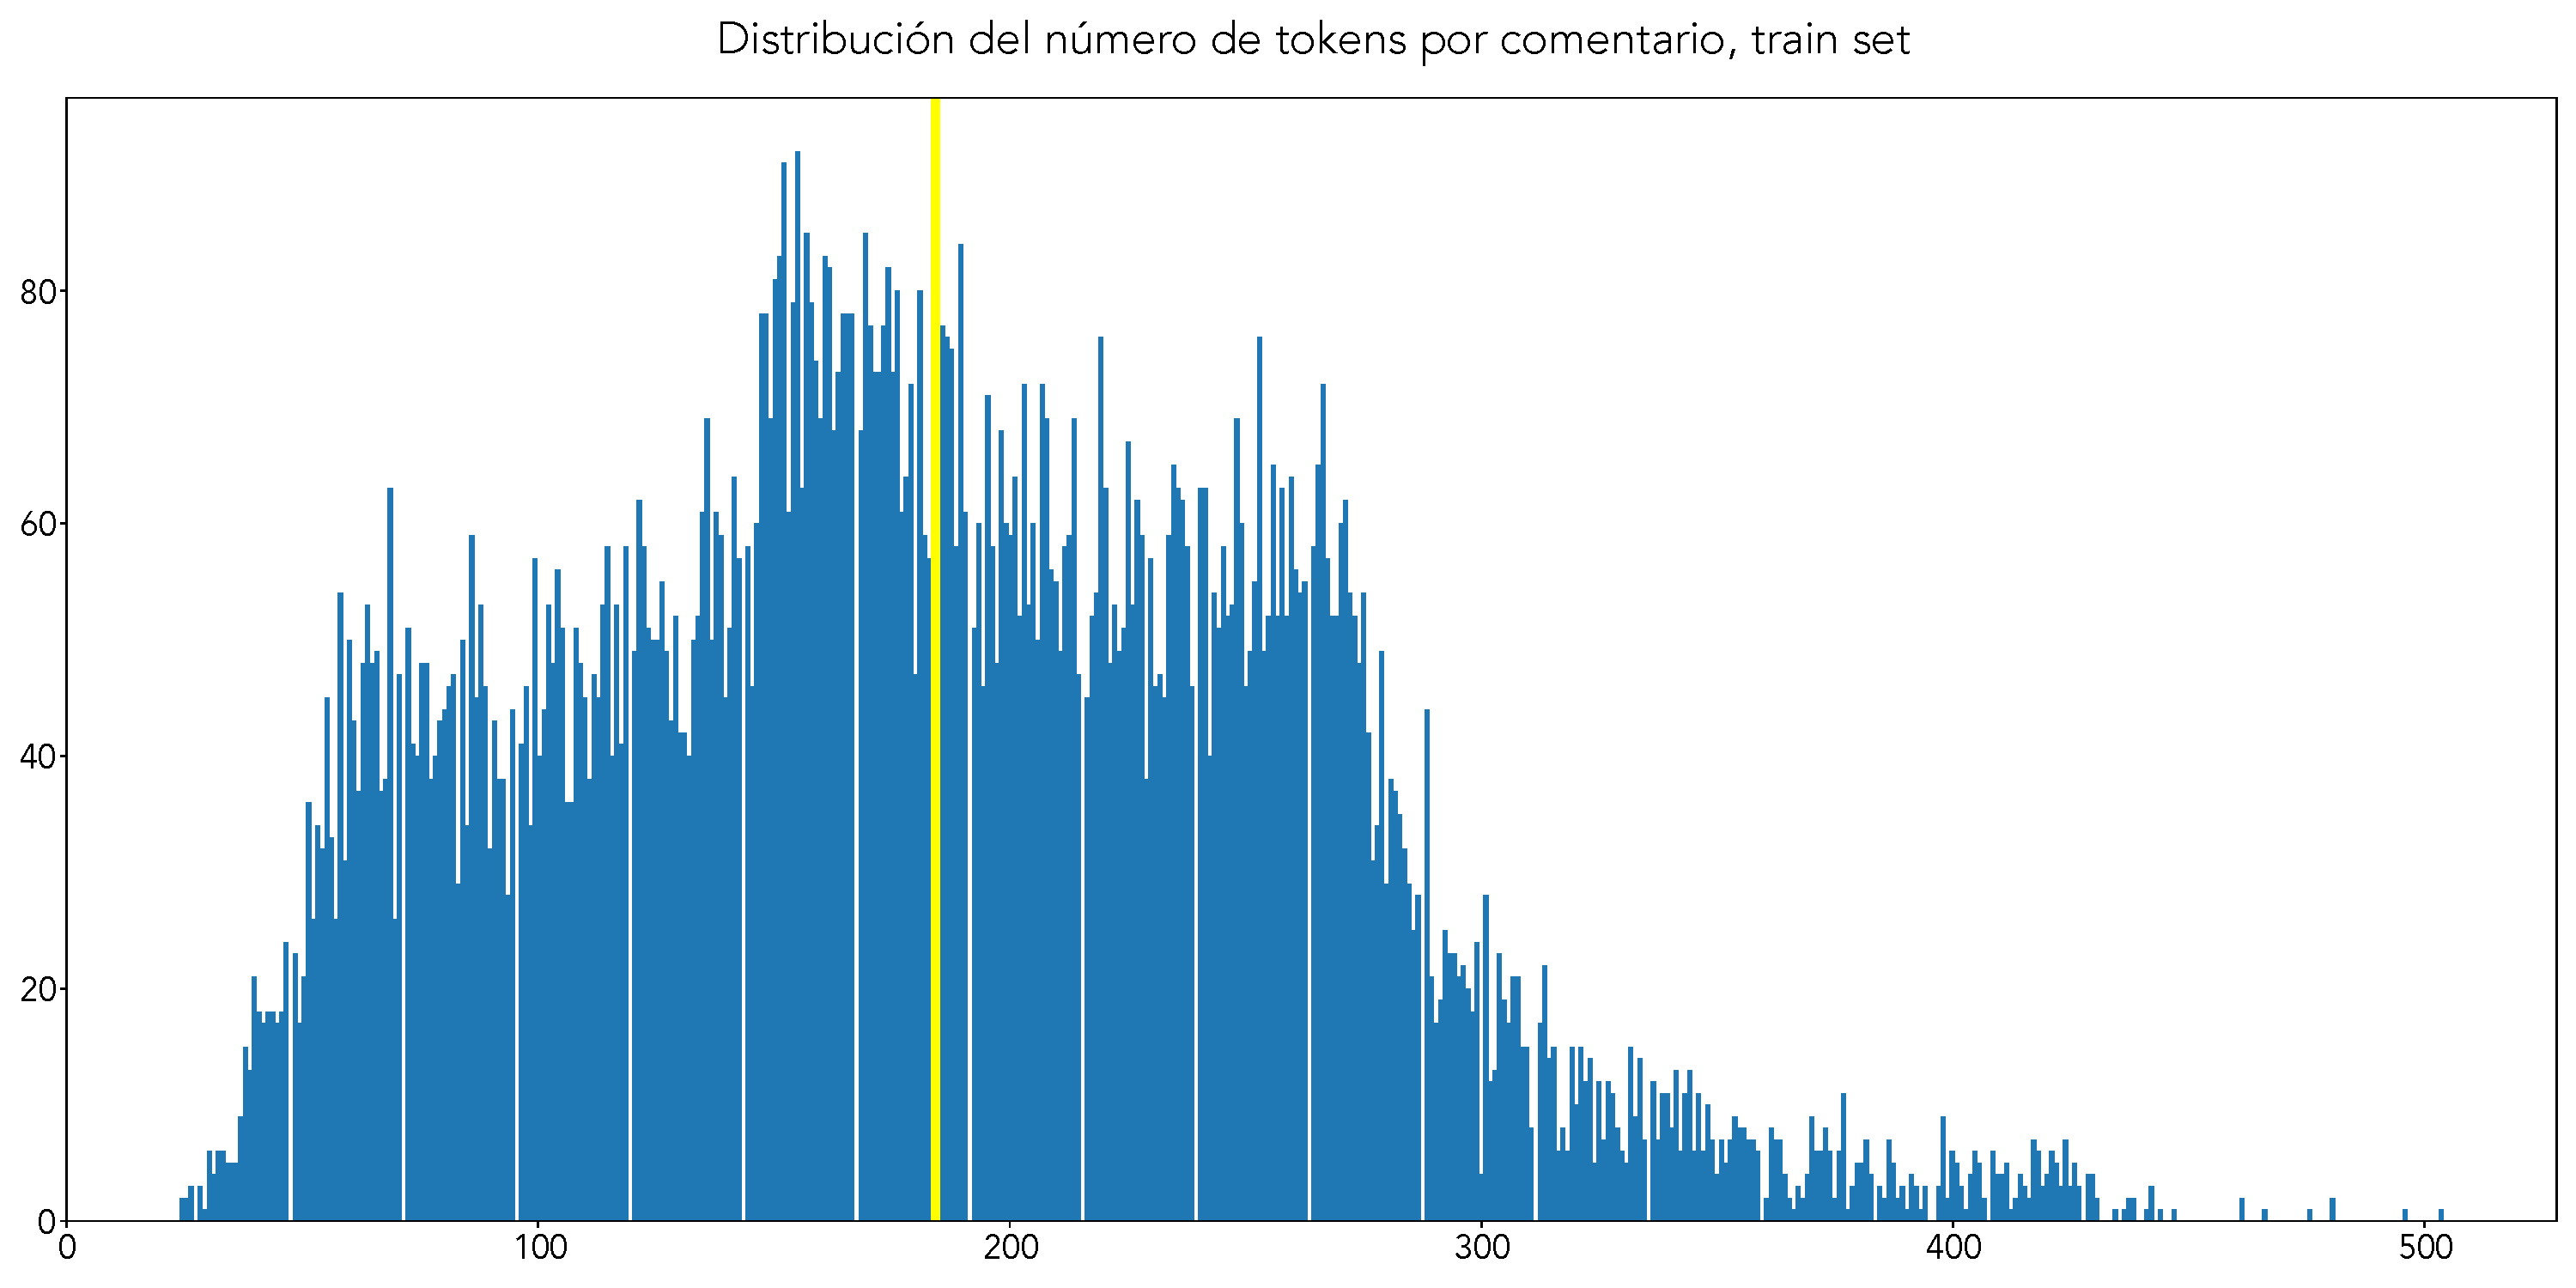
\includegraphics[width=.9\textwidth]{media/tokens_hist_train.pdf}
		\caption{Distribución del número de tokens por comentario en el conjunto de entrenamiento}
		\label{fig:avg_tokens_train}
	\end{subfigure}

	\caption{Visualización de la distribución de nuestro conjunto de entrenamiento}
	\label{fig:sum_train}
\end{figure}


\begin{figure}[h!]
	\centering
	\begin{subfigure}[t]{0.95\textwidth}
		\centering
		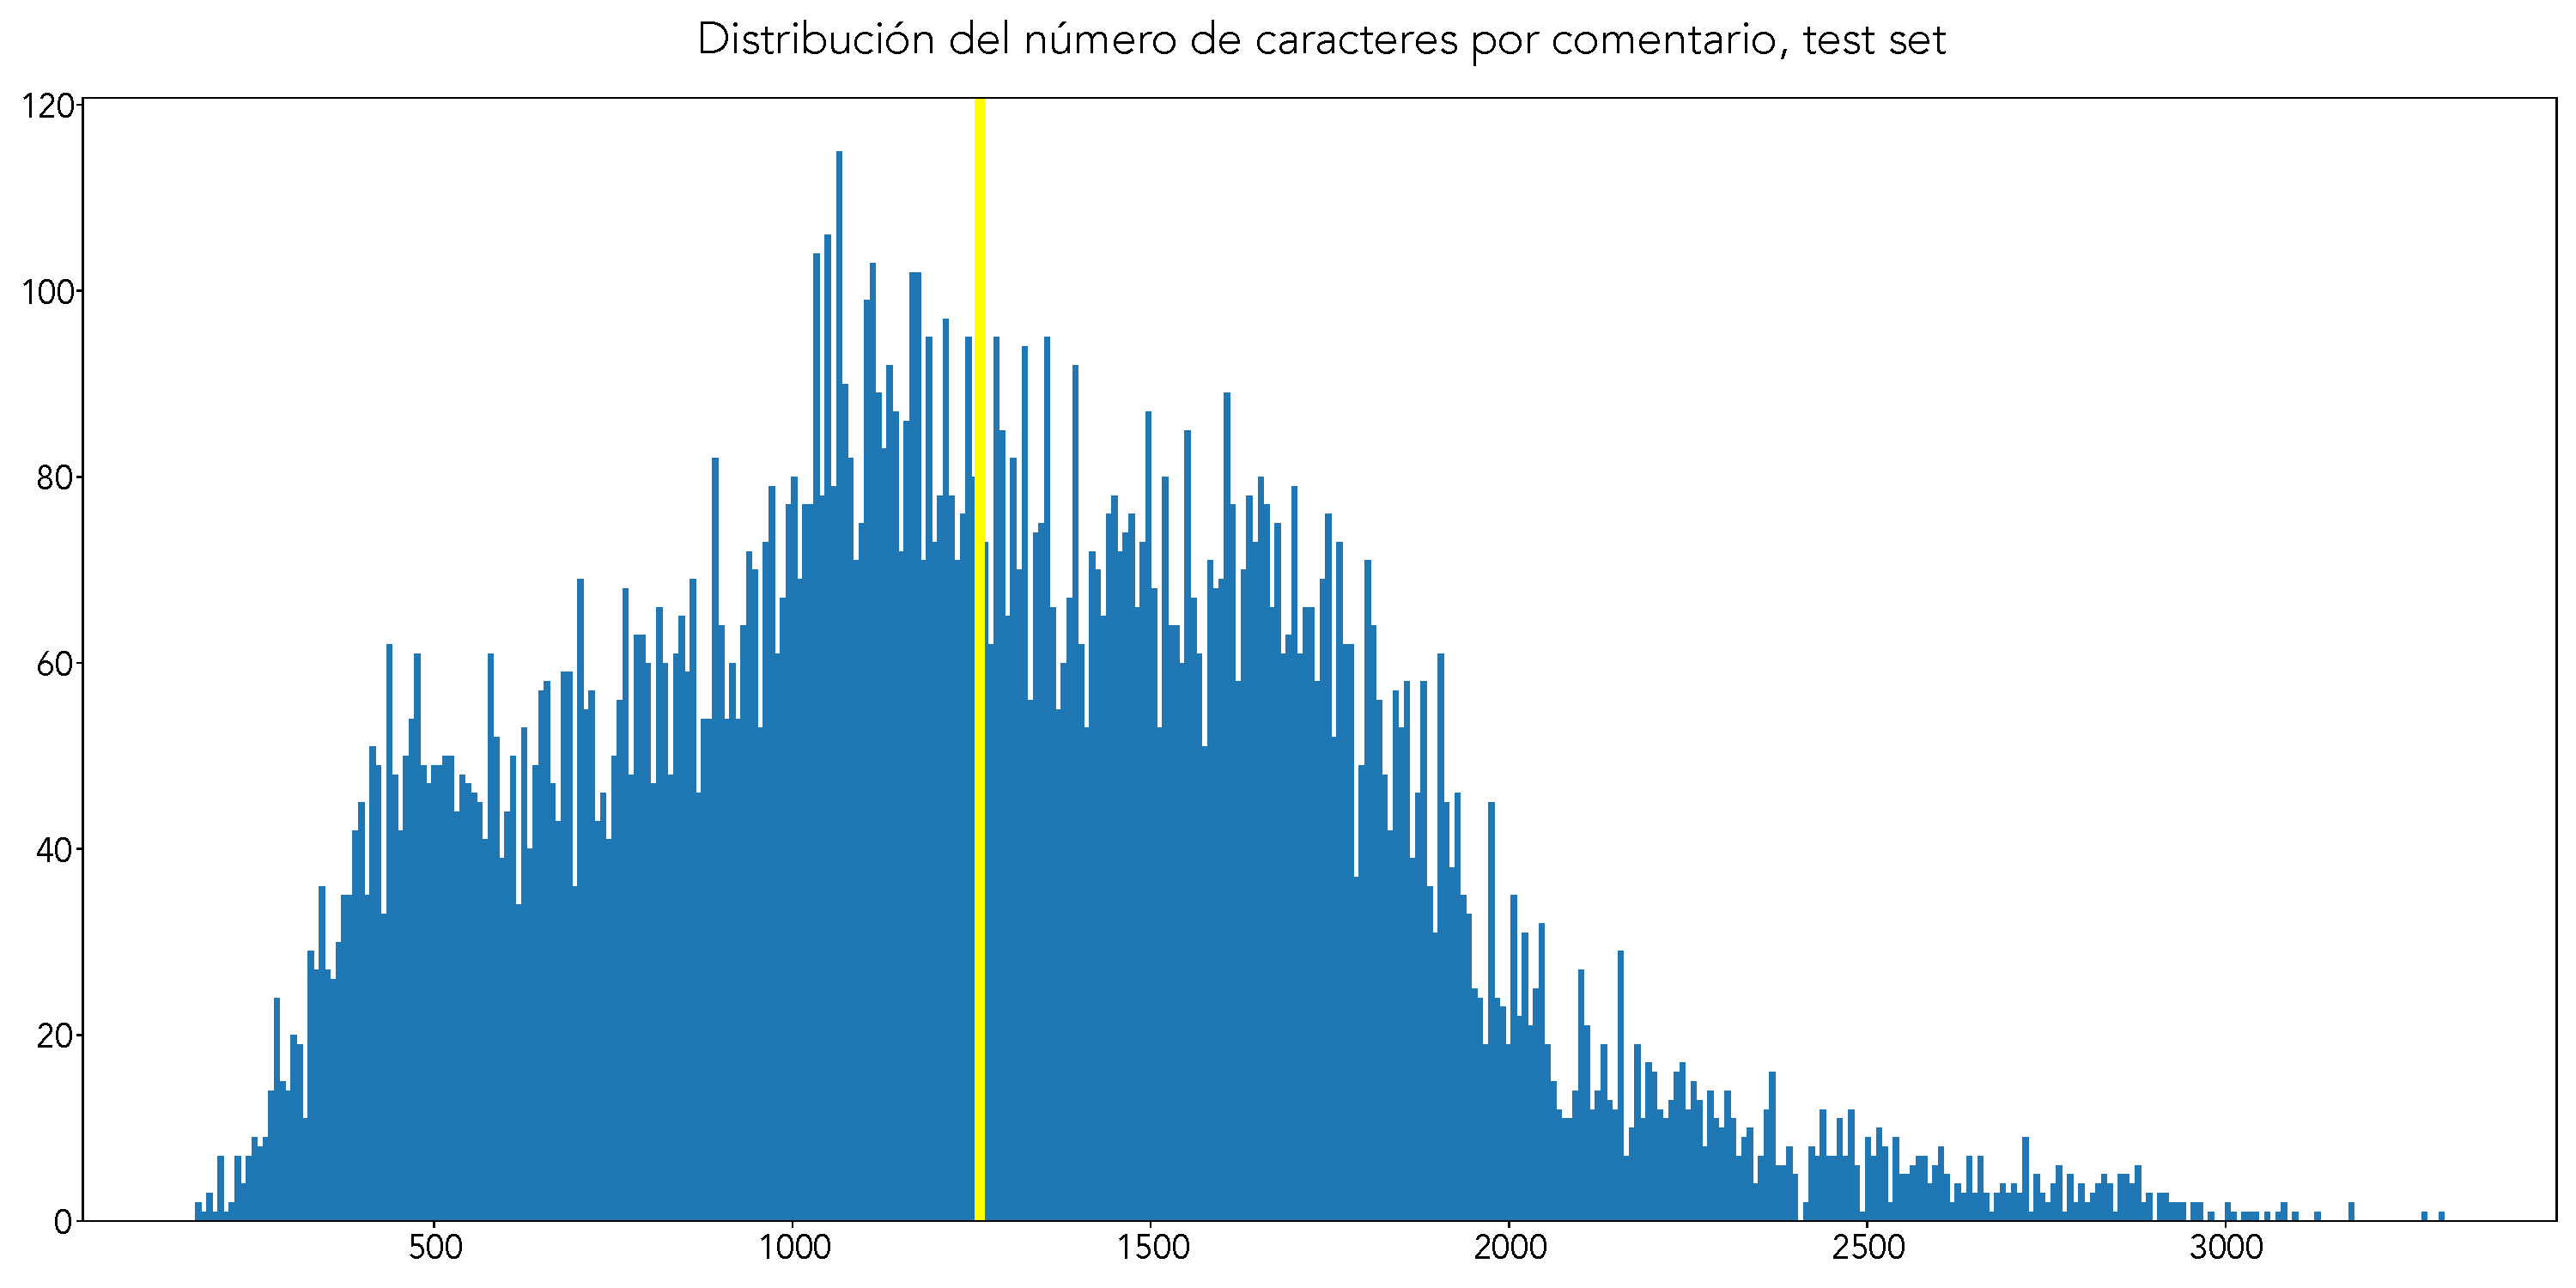
\includegraphics[width=.9\textwidth]{media/char_hist_test.pdf}
		\caption{Distribución del número de caracteres por comentario, en el conjunto de evaluación}
		\label{fig:avg_char_test_test}
	\end{subfigure}

	~

	\begin{subfigure}[t]{0.95\textwidth}
		\centering
		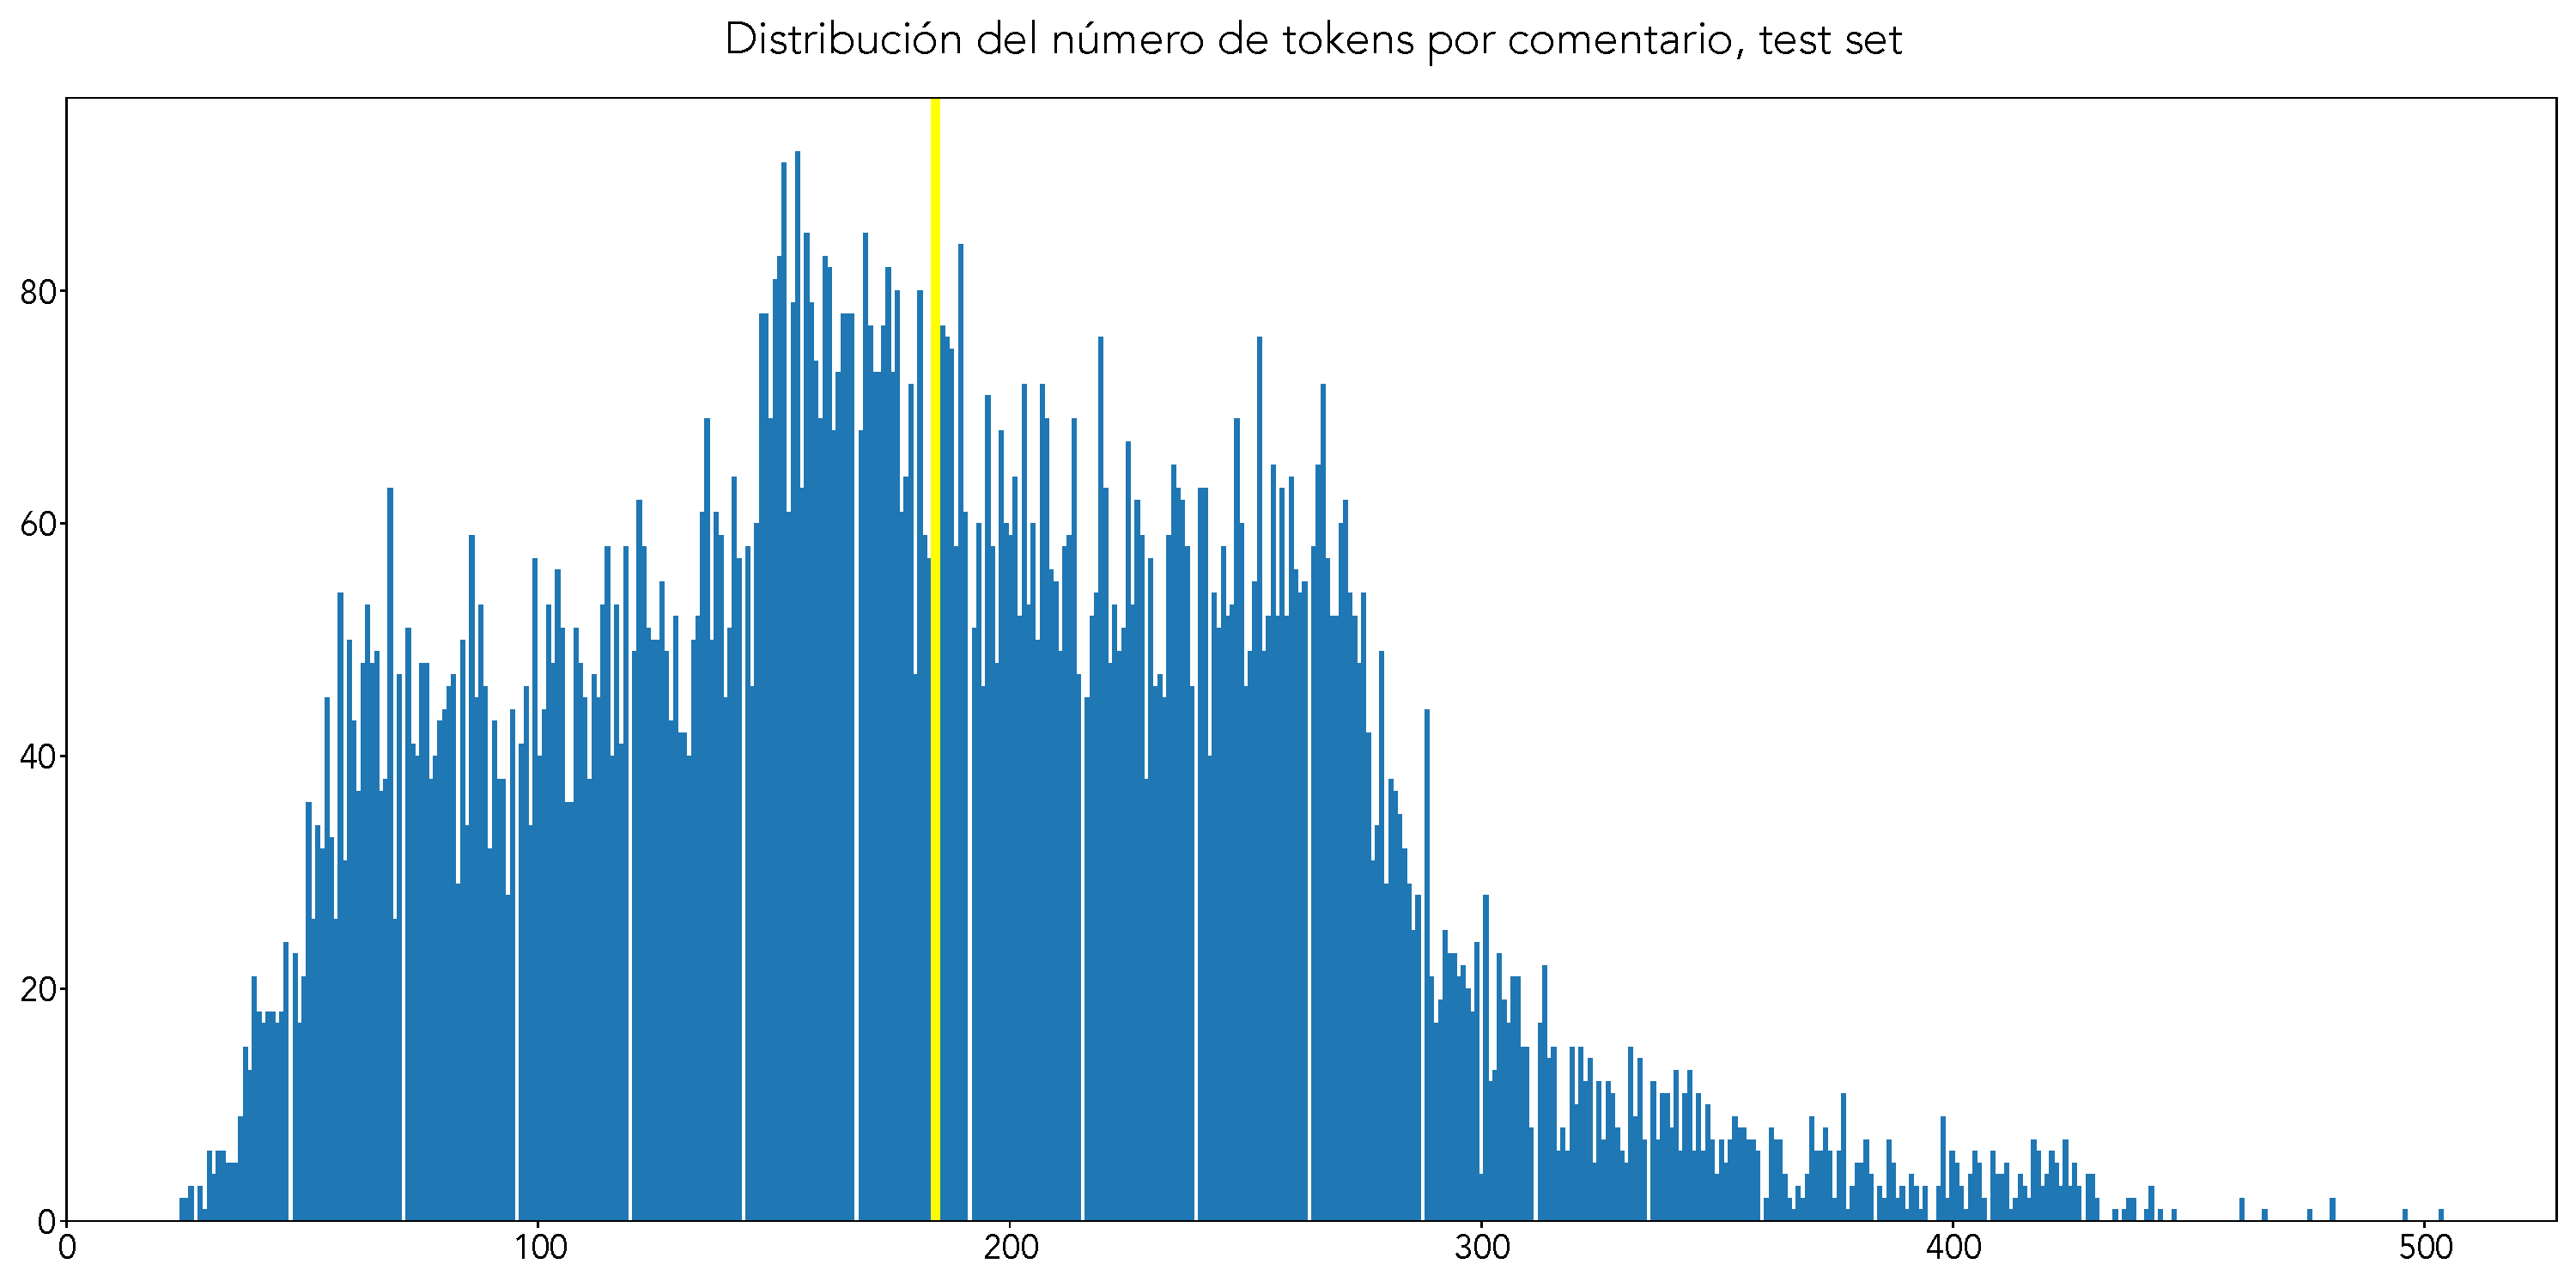
\includegraphics[width=.9\textwidth]{media/tokens_hist_test.pdf}
		\caption{Distribución del número de tokens por comentario en el conjunto de evaluación}
		\label{fig:avg_tokens_test}
	\end{subfigure}


	\caption{Visualización de la distribución de nuestro conjunto de evaluación}
	\label{fig:sum_test}
\end{figure}

Una media de casi 200 palabras por comentario con comentarios alcanzando las 500 corresponde con comentarios relativamente largos. Esto nos vendrá bien de cara al entrenamiento de nuestro modelo, para poder formar oraciones con más sentido.


\subsection{Dataset: \textit{Medical Transcriptions}}
Este dataset es en realidad una extracción de la página web \url{mtsamples.com}, donde se halla una respetable cantidad de trasncripciones médicas. La autora extrajo todos los comentarios, así como los diferentes metadatos que los acompañaban mediante \textit{web scraping} y los provee en la columna \jesitt{trasncription}.

Al igual que el anterior, este conjunto de datos se corresponde con informes de operaciones quirúrgicas en inglés, y de igual forma anonimizado.

En este caso, como podemos apreciar en la Figura \ref{fig:sum_mdtr}, las distribuciones son ligeramente asimétricas, predominando comentarios más cortos. Aún así, disponemos de comentarios excepcionalmente largos, con alrededor de 18000 caracteres.

\begin{figure}[h!]
	\centering
	\begin{subfigure}[t]{0.95\textwidth}
		\centering
		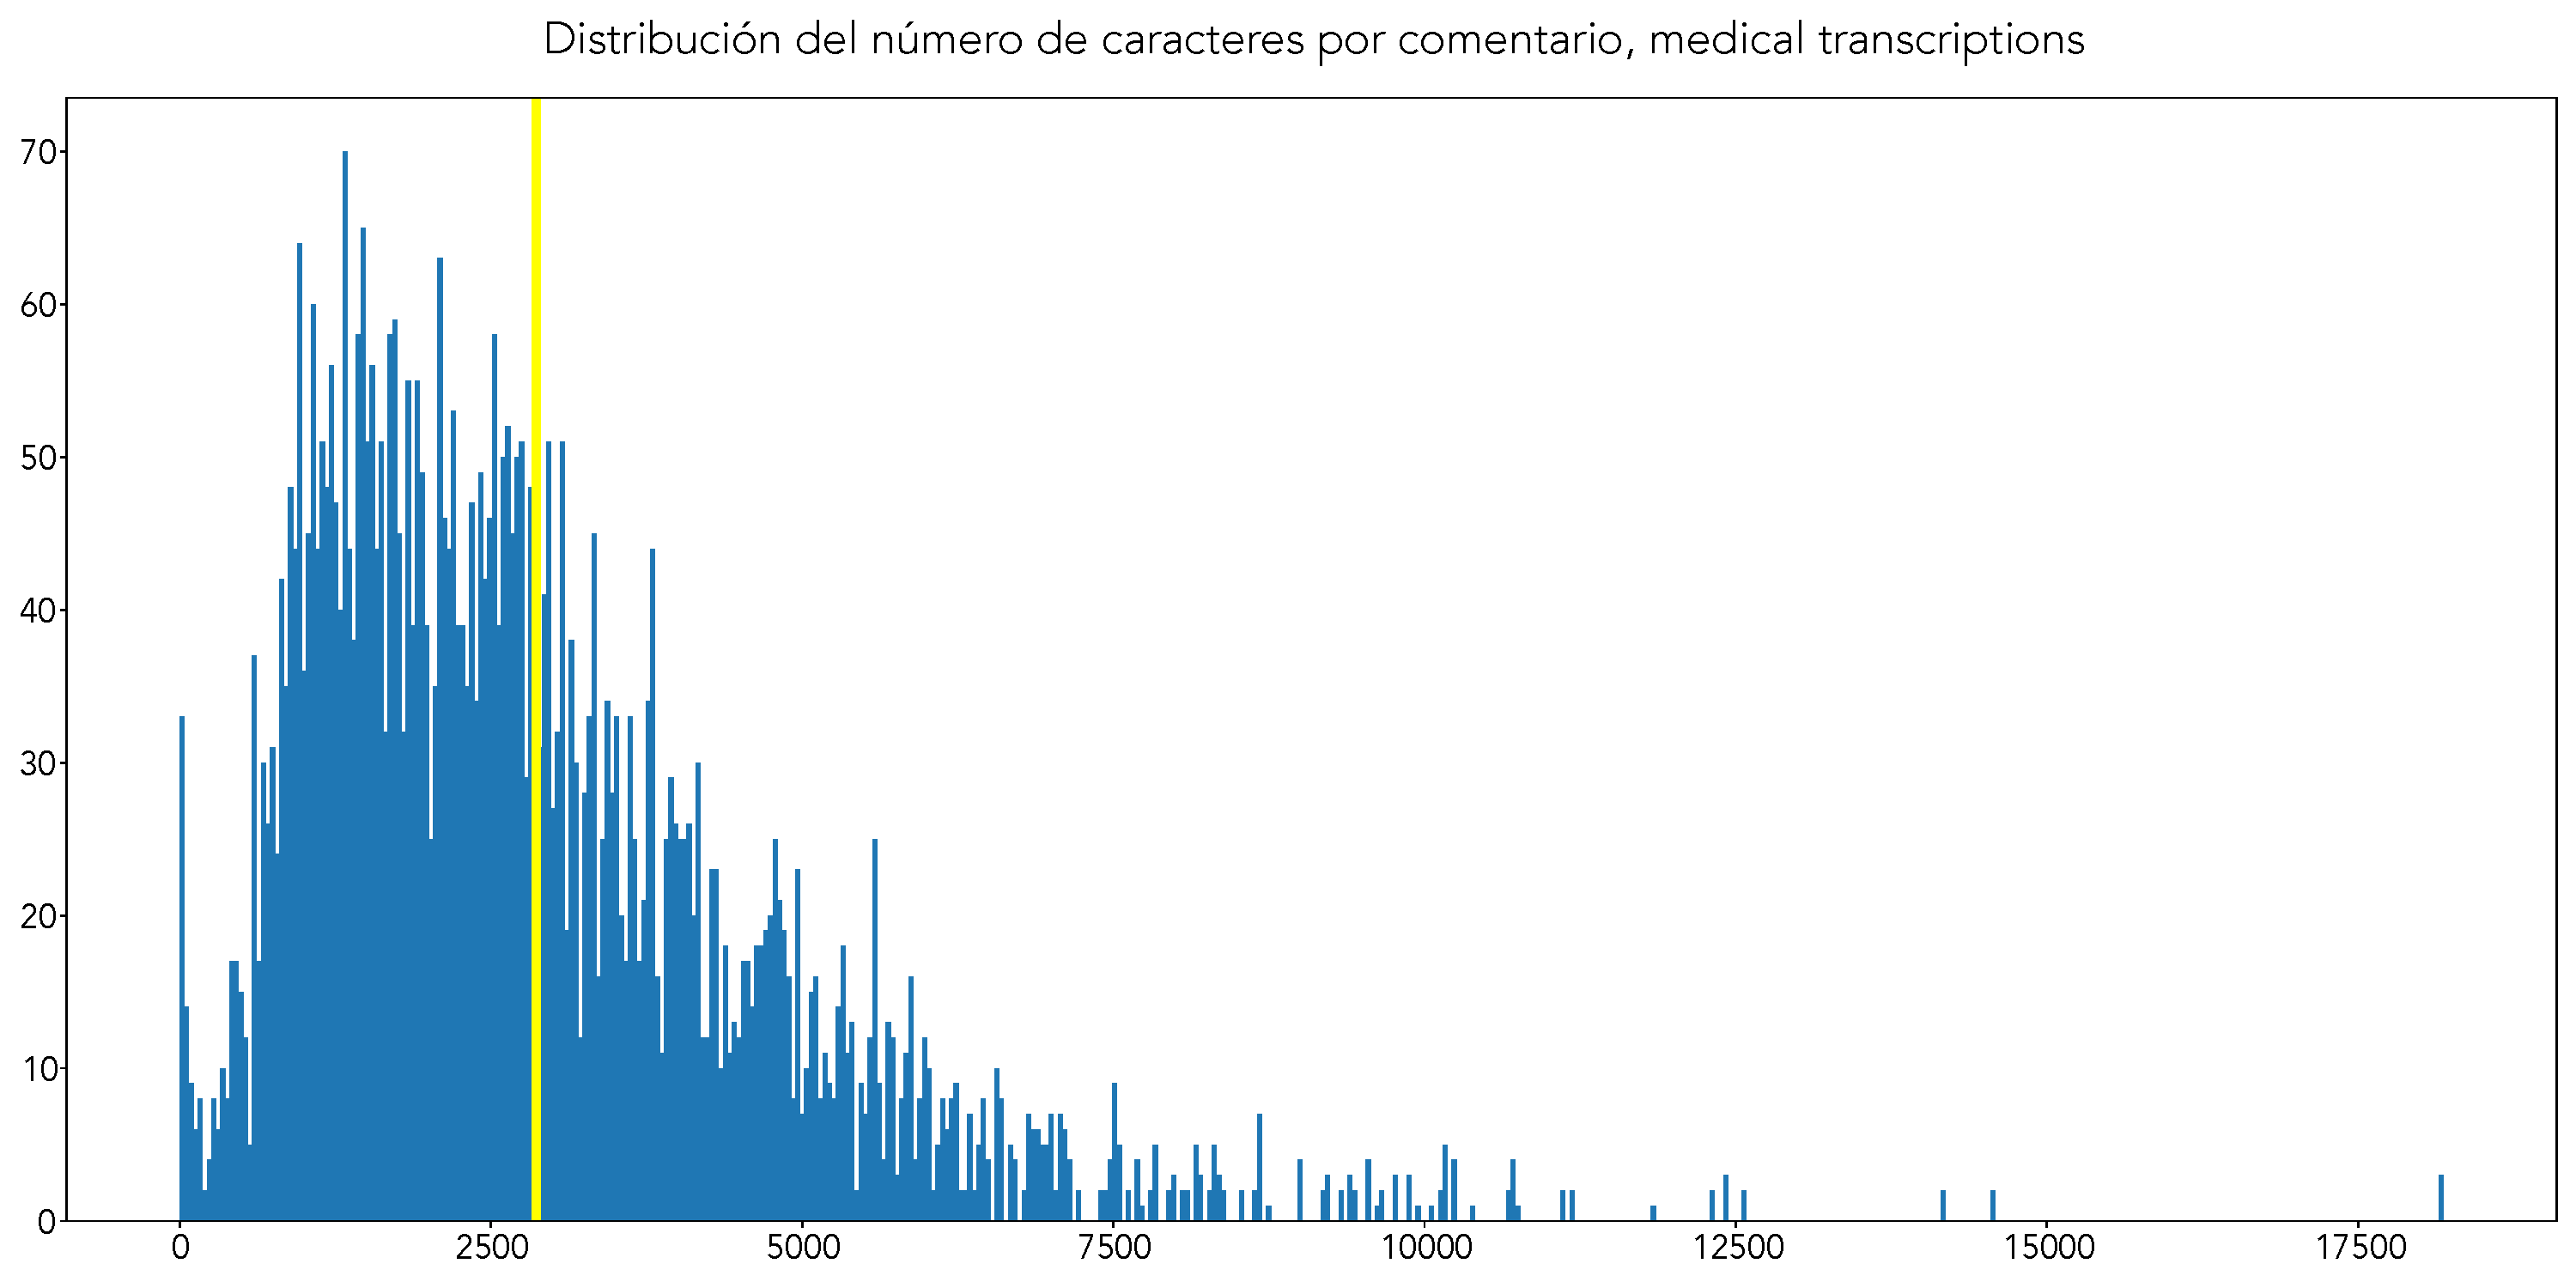
\includegraphics[width=.9\textwidth]{media/char_hist_mdtr.pdf}
		\caption{Distribución de caracteres en el dataset Medical Transcriptions}
		\label{fig:char_hist_mdtr}
	\end{subfigure}

	~
	\begin{subfigure}[t]{0.95\textwidth}
		\centering
		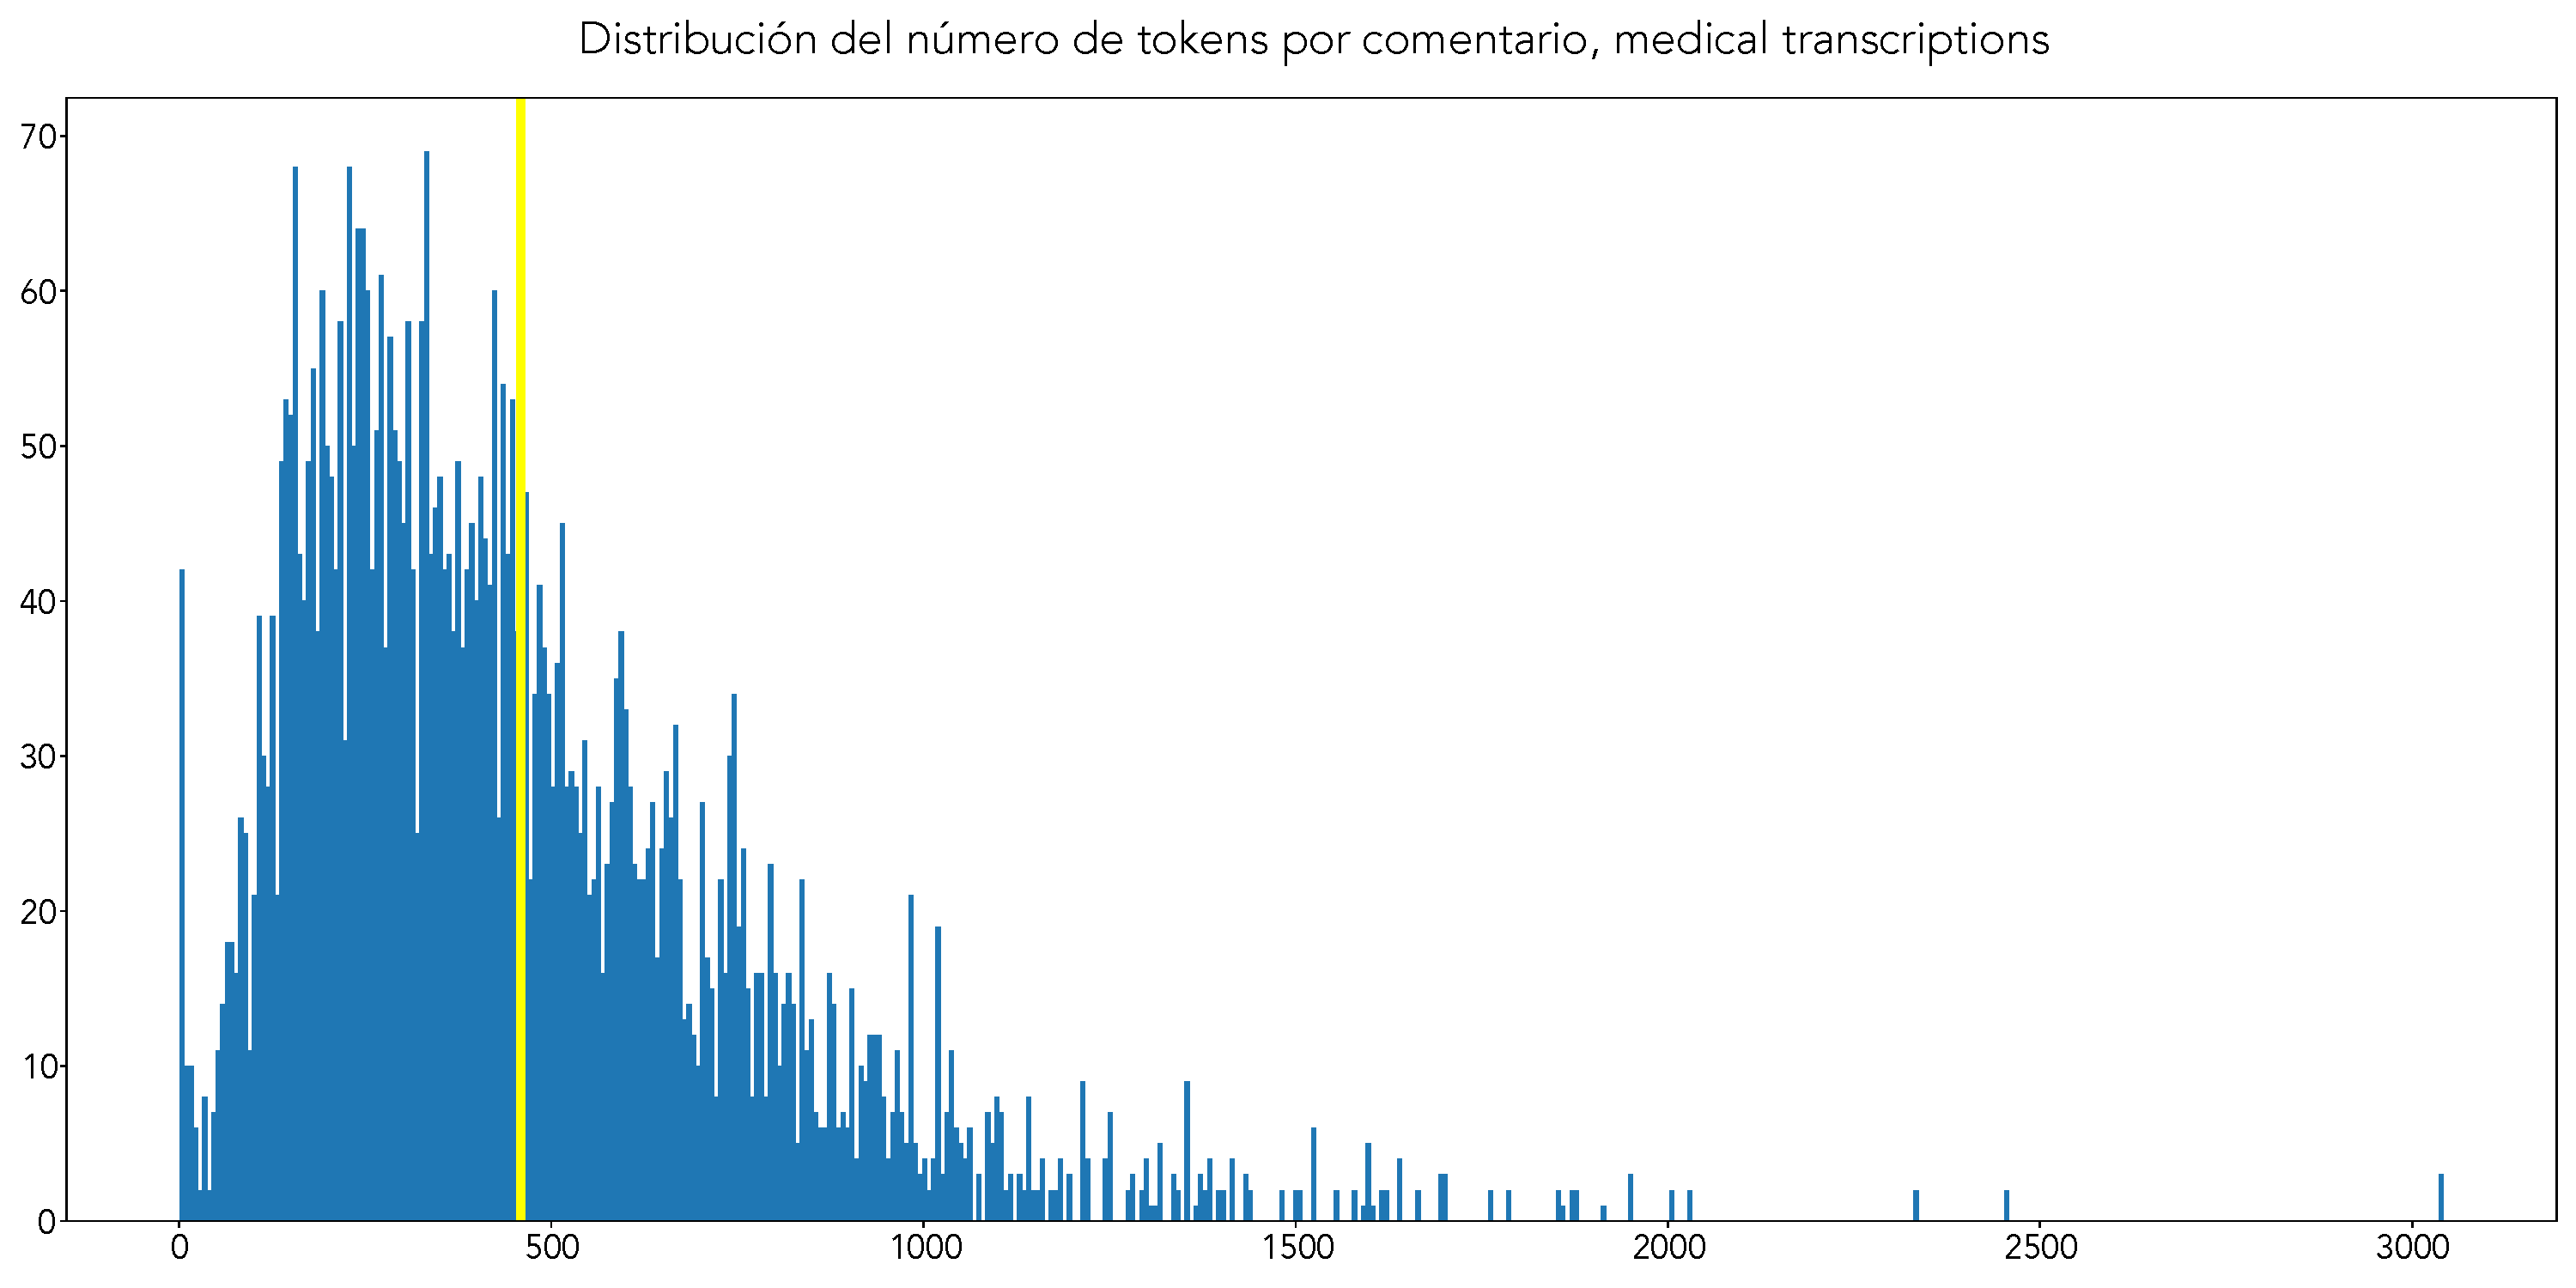
\includegraphics[width=.9\textwidth]{media/token_hist_mdtr.pdf}
		\caption{Distribución de palabras en el dataset Medical Transcriptions}
		\label{fig:token_hist_mdtr}
	\end{subfigure}

	\caption{Visualización del dataset Medical Transcriptions}
	\label{fig:sum_mdtr}
\end{figure}



\section{Preprocesamiento}
\label{sec:preprocess}
En esta sección, describiremos el preprocesamiento acometido en cada uno de los datsets. Provienen de fuentes diferentes así que cada uno recibirá un trato diferente, con objeto de normalizar y unificar el formato de todos de cara al entrenamiento.




\subsection{Medical Text}
Este conjunto de datos, siendo específicamente texto, el formato, ortografía y en general formato de los archivos es muy bueno. Simplemente hemos de eliminar las categorías adjuntas a cada comentario, para obtener una lista de comentarios crudos en sí. Por lo demás, los comentarios carecen de problemas de formato, codificación o cualquier otra cosa que pudiera interferir con el proceso de entrenamiento. Probablemente el autor ya hiciera esto por nosotros antes de publicarlo.


\subsection{Medical Transcriptions}
En el caso de las trancripciones médicas, la tarea es considerablemente más compleja. El conjunto de datos proviene de la página web \url{mtsamples.com}, como especificamos anteriomente. La autora efectuó un proceso de \textit{web scraping} para obtener toda la información y recogerla en el archivo \jesitt{.csv}. 

Esto facilita las cosas, pero desde luego los comentarios deben ser tratados en profundidad antes de poder pasarlos a cualquier modelo. Los trazos de formato en HTML se dejan entrever en los comentarios con signos de puntuación o tabulaciones fuera de lugar, apreciables en el Comentario \ref{com:mt-before}, así que debemos arreglarlo previo entrenamiento.

Para ello, se ha hecho un fuerte uso de expresiones regulares, y se ha creado un \textit{pipeline} para procesar todo el texto a la vez.

El pipeline elimina todas las posibles trazas o residuos que hubieran quedado del \textit{web scraping}. Podemos ver el pipeline diseñado en la Figura \ref{code:pipeline-regex-mdtr} del Apéndice.

El resumen del proceso es eliminar signos de puntuación mal colocados, eliminar títulos o cabeceras de secciones de la página web, sustituir múltiples espacios por uno solo o eliminar los números de listas enumeradas (1., 2., etc). Finalmente, se añaden las etiquetas que vemos en la Figura \ref{fig:preprocess-diagram}. Se explicará su funcionamiento en la sección de la experimentación.

El resultado es un texto muy limpio y claro, mucho más apto para la fase de entrenamiento.

Podemos ver una comparativa del antes (Comentario \ref{com:mt-before}) y el después (Comentario \ref{com:mt-after}) del preprocesamiento de un determinado comentario de nuestro dataset. Los comentarios han sido truncados debido a su longitud.


\begin{thm}
	\sffamily{
		\small{
		SUBJECTIVE:,  This 23-year-old white female presents with complaint of allergies.  She used to have allergies when she lived in Seattle but she thinks they are worse here.  In the past, she has tried Claritin, and Zyrtec.  Both worked for short time but then seemed to lose effectiveness.  She has used Allegra also.  She used that last summer and she began using it again two weeks ago. [...]
		}
	}
	\label{com:mt-before}
\end{thm}


\begin{thm}
	\sffamily{
		\small{
		$<|$ BOS $|>$This 23-year-old white female presents with complaint of allergies. She used to have allergies when she lived in Seattle but she thinks they are worse here. In the past, she has tried Claritin, and Zyrtec. Both worked for short time but then seemed to lose effectiveness. She has used Allegra also. She used that last summer and she began using it again two weeks ago. [...] $<|$ EOS $|>$}
	}
	\label{com:mt-after}
\end{thm}


Tras haber preprocesado y cribado todos los elementos que pudieran suponer un problema a la hora de entrenar nuestro modelo, lo que obtenemos es un dataset unificado con un total de 33846 comentarios, sumando un total de 7537697 palabras con una media de 222 tokens y 1482 caracteres por comentario. 


Vemos además, en la Figura \ref{fig:wordcloud} una nube de palabras de todo el conjunto de datos. 

\begin{figure}[h]
	\centering
	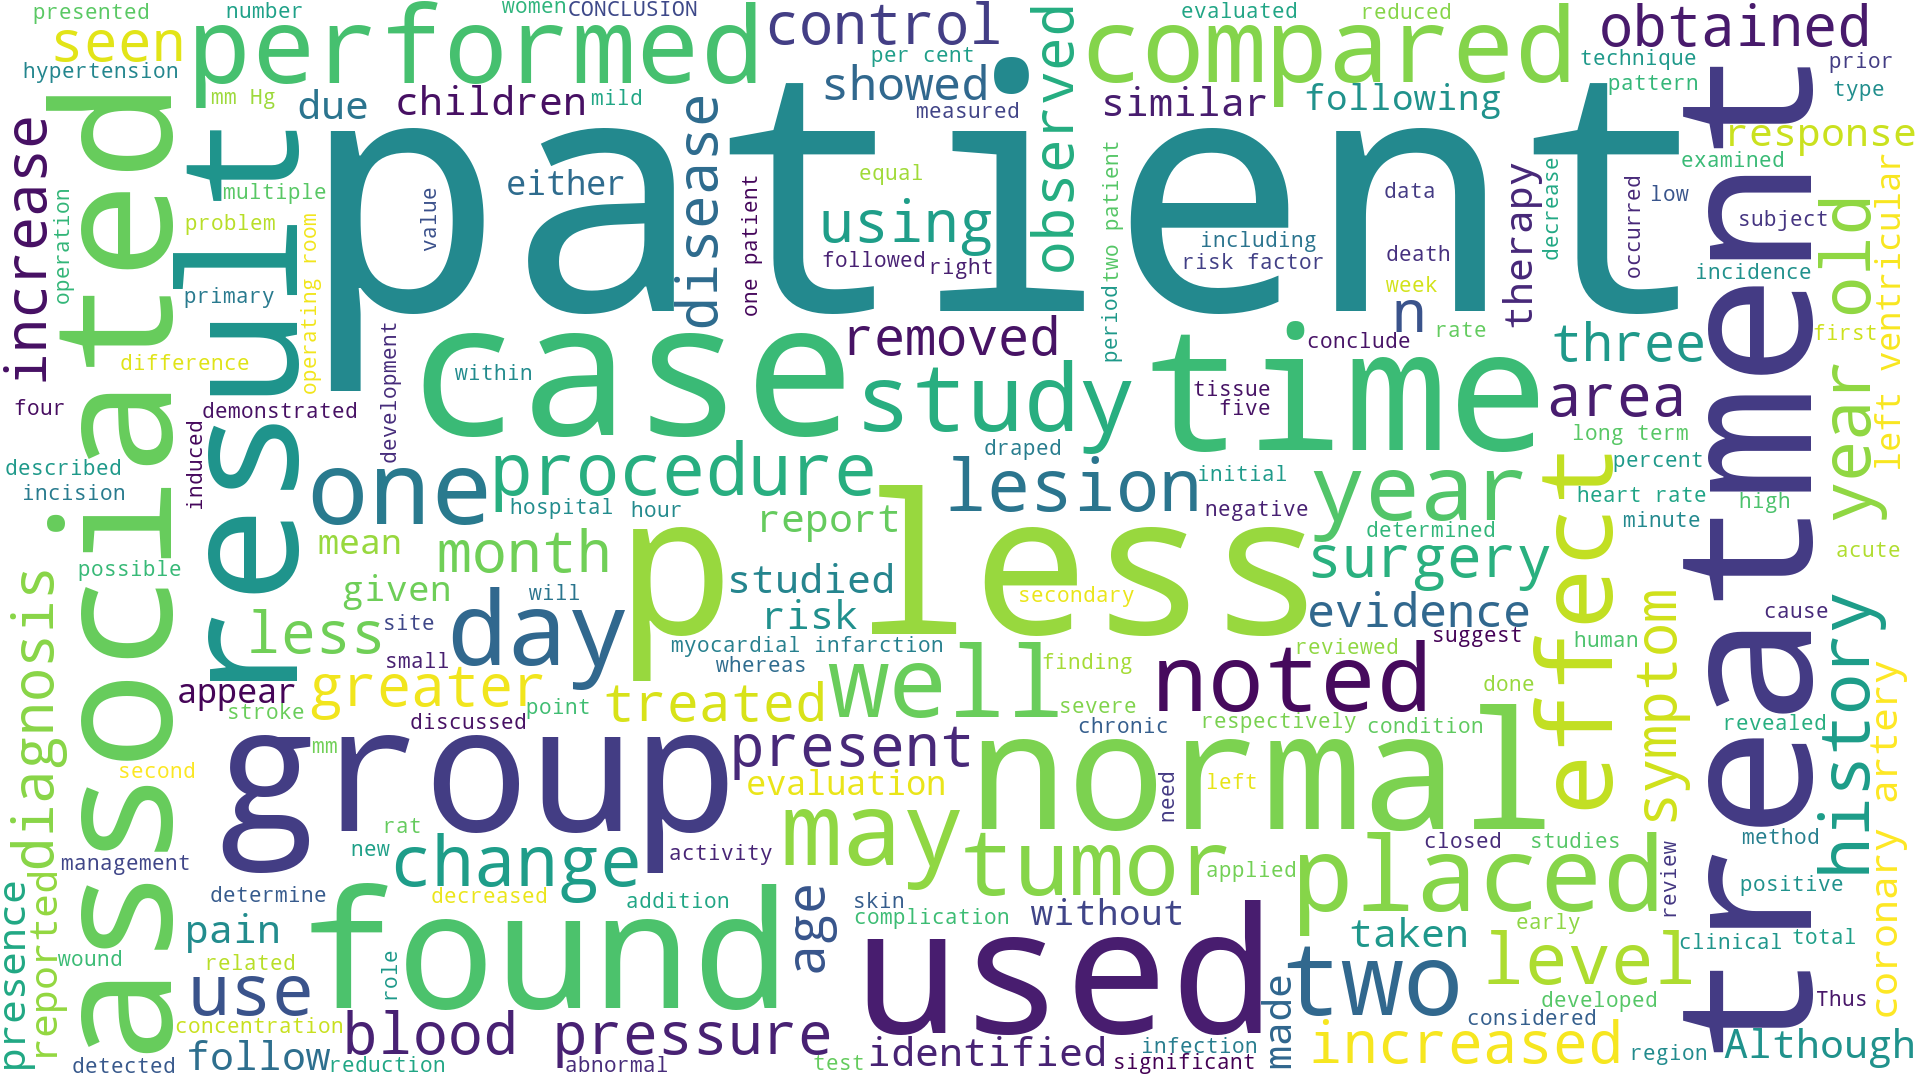
\includegraphics[width=.9\textwidth]{media/wordcloud_full_data.png}
	\caption{Wordcloud de todo el conjunto de datos}
	\label{fig:wordcloud}
\end{figure}

Se aprecia que las palabras más comunes son \textit{patient}, \textit{case}, o \textit{treatment}, junto con \textit{study} o \textit{performed}. Esta nube de palabras se ha calculado en el texto preprocesado, pero el preprocesamiento solo ha tenido en cuenta cuestiones de formato, mayoritariamente. De ahí que términos como \textit{used}, \textit{using} o \textit{use} aparezcan a la vez. No hemos hecho stemming ni lemmatization porque nos interesa el contenido de las oraciones tal y como está, que es como el modelo fue diseñado para ser entrenado.

Disponiendo de este dataset, estamos listos para poder entrenar y ajustar nuestro modelo para que genere comentarios muy similares a los presentes en nuestro conjunto de datos.